\section{MODELLING}
\begin{frame}{\secname}
\end{frame}

\subsection{Decision Tree}

\begin{frame}{\subsecname\ : Baselines(s)}

The first model tested was a \txt{DecisionTreeClassifier}, which was also used to fine-tune the method used for subsequent estimators. From figure \ref{fig:DT_base_overs}, we see that using the oversampled data already produced a slight improvement.

\begin{figure}
    \centering
    \begin{subfigure}[c]{0.4\textwidth}
        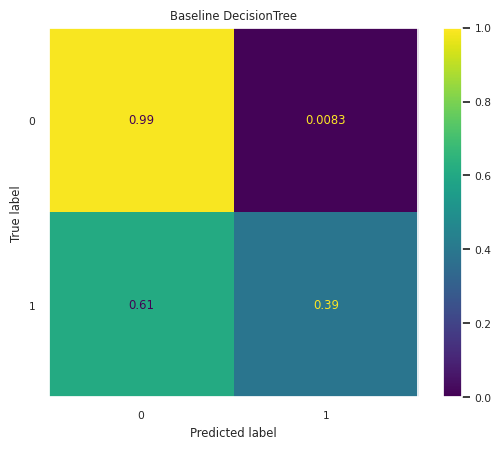
\includegraphics[width=\textwidth]{images/models/DT_base.png}
        \caption{Using the original dataset}
        \label{fig:DT_base}
    \end{subfigure}
    \begin{subfigure}[c]{0.4\textwidth}
        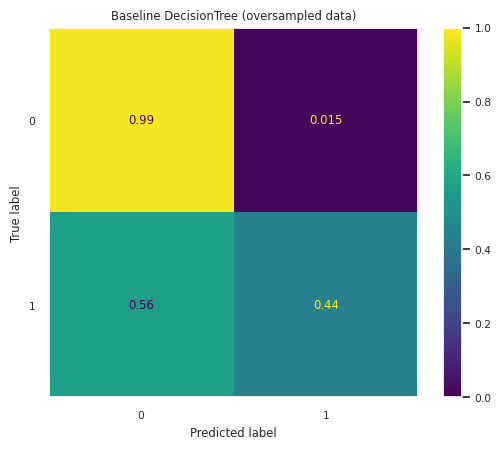
\includegraphics[width=\textwidth]{images/models/DT_base_overs.png}
        \caption{Using oversampled dataset}
        \label{fig:DT_base_overs}
    \end{subfigure}
    \caption{\txt{DecisionTreeClassifier} baselines}
    \label{fig:DT_bases}
\end{figure}
\end{frame}

\begin{frame}{\subsecname\: Grid search}
\begin{columns}[t]
    \column{0.37\textwidth}
    \justifying
    After confirming the choice of using the oversampled data, a grid search for each of the four main scoring metrics shows that the one we should focus on is \txt{recall_macro}, see figure \ref{fig:DT_recmacro}, which will be used for all subsequent tunings.

    This is because it "requires" a model that correctly classifies as many classes as possible, giving more importance to the minority.
    \column{0.63\textwidth}
        \begin{figure}
            \centering
            \vspace{-2.0em} 
            \begin{columns}[t]
                \column{.5\textwidth}
                    \centering
                    \begin{subfigure}[c]{\textwidth}
                        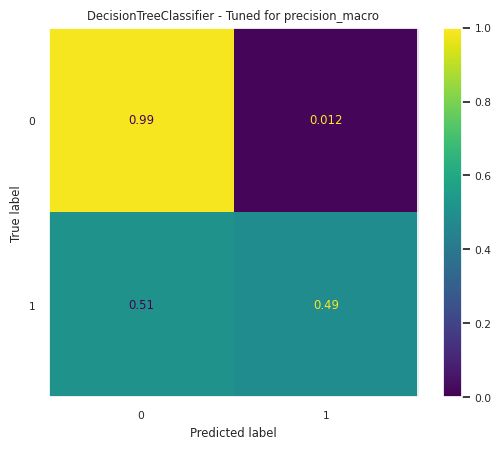
\includegraphics[width=\textwidth]{images/models/DT_precmacro.png}
                        \caption{\txt{precision_macro}}
                        \label{fig:DT_precmacro}
                    \end{subfigure} \\
                    \vspace{-.4em} 
                    \begin{subfigure}[c]{\textwidth}
                        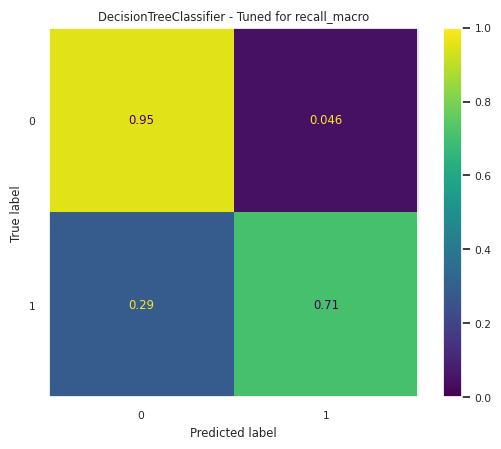
\includegraphics[width=\textwidth]{images/models/DT_recmacro.png}
                        \caption{\txt{recall_macro}}
                        \label{fig:DT_recmacro}
                    \end{subfigure}
                \column{.5\textwidth}
                    \centering
                    \begin{subfigure}[c]{\textwidth}
                        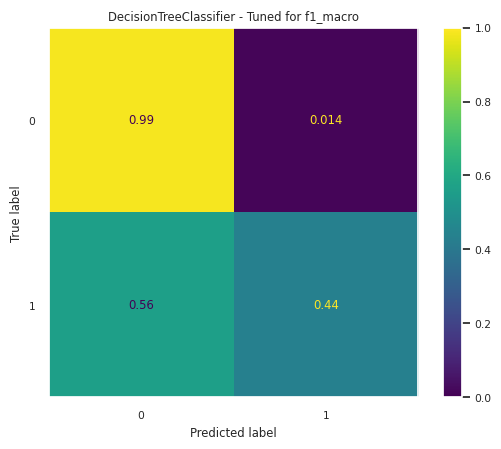
\includegraphics[width=\textwidth]{images/models/DT_f1macro.png}
                        \caption{\txt{f1_macro}}
                        \label{fig:DT_f1macro}
                    \end{subfigure} \\
                    \vspace{-.4em} 
                    \begin{subfigure}[c]{\textwidth}
                        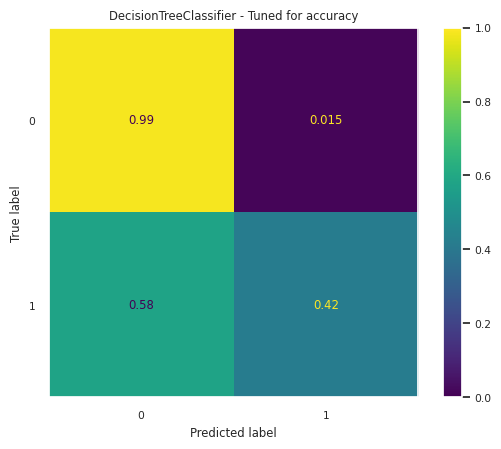
\includegraphics[width=\textwidth]{images/models/DT_acc.png}
                        \caption{\txt{accuracy}}
                        \label{fig:DT_acc}
                    \end{subfigure}
            \end{columns}
            \vspace{-0.8em} 
            %\caption{Tuned results for each metric}
            \label{fig:DT_grids}
        \end{figure}
\end{columns}

\end{frame}

\begin{frame}{\subsecname : Final results}
\begin{columns}
    \column{0.5\textwidth}
    \begin{table}
        \footnotesize
        \centering
        \begin{tabular}{ll}
            parameter & tuned value \\
            \hline\hline
            \txt{max_depth} & 14 \\
            \txt{criterion} & \txt{"gini"} \\
            \txt{class_weight} & \txt{"balanced"} \\
        \end{tabular}
        %\label{tab:my_label}
    \end{table}
    \column{0.5\textwidth}
    \begin{table}
        \footnotesize
        \centering
        \begin{tabular}{lc}
            metric & result \\
            \hline\hline
            \txt{recall} (class 1) & 71\% \\
            \txt{recall_macro} & 83\% \\
        \end{tabular}
        %\label{tab:my_label}
    \end{table}
\end{columns}

\begin{figure}
    \centering
    \begin{subfigure}[c]{0.4\textwidth}
        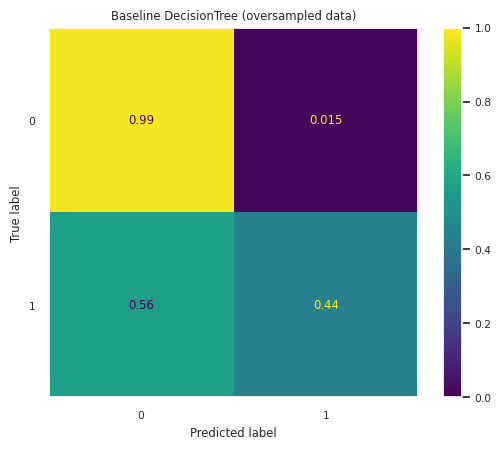
\includegraphics[width=\textwidth]{images/models/DT_base_overs.png}
        \caption{Baseline}
        \label{fig:DT_baseline}
    \end{subfigure}
    \begin{subfigure}[c]{0.4\textwidth}
        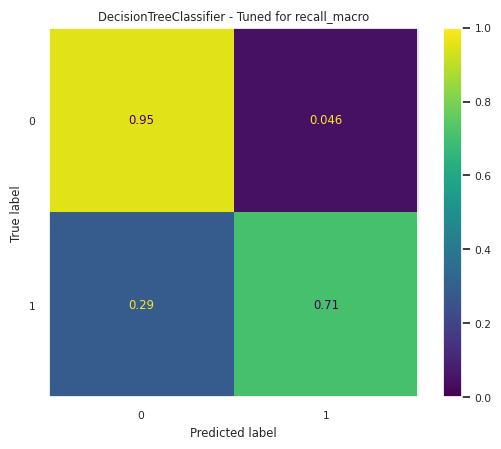
\includegraphics[width=\textwidth]{images/models/DT_recmacro.png}
        \caption{Tuned}
        \label{fig:DT_tuned}
    \end{subfigure}
    \caption{\subsecname\ results}
    \label{fig:DT_results}
\end{figure}
\end{frame}

\subsection{Random Forest}

\begin{frame}{\subsecname}
\begin{columns}
    \column{0.5\textwidth}
    \begin{table}
        \footnotesize
        \centering
        \begin{tabular}{ll}
            parameter & tuned value \\
            \hline\hline
            \txt{max_depth} & 9 \\
            \txt{criterion} & \txt{"gini"} \\
            \txt{class_weight} & \txt{"balanced"} \\
            \txt{n_estimators} & 100
        \end{tabular}
        %\label{tab:my_label}
    \end{table}
    \column{0.5\textwidth}
    \begin{table}
        \footnotesize
        \centering
        \begin{tabular}{lc}
            metric & result \\
            \hline\hline
            \txt{recall} (class 1) & 84\% \\
            \txt{recall_macro} & 89\% \\
        \end{tabular}
        %\label{tab:my_label}
    \end{table}
\end{columns}

\begin{figure}
    \centering
    \begin{subfigure}[c]{0.4\textwidth}
        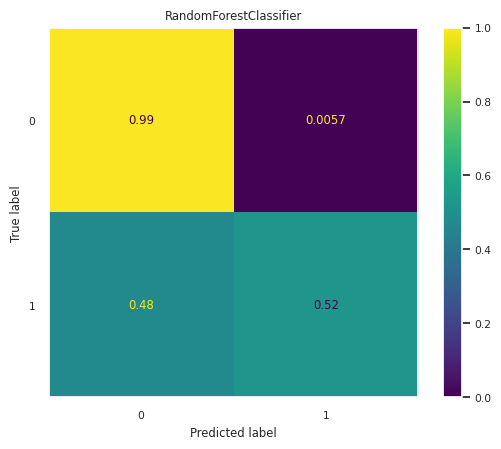
\includegraphics[width=\textwidth]{images/models/RF_base.png}
        \caption{Baseline}
        \label{fig:RF_base}
    \end{subfigure}
    \begin{subfigure}[c]{0.4\textwidth}
        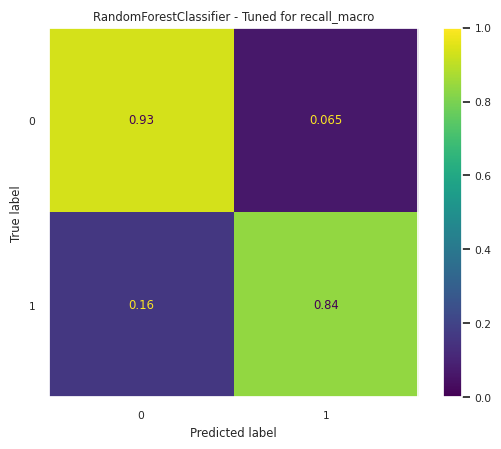
\includegraphics[width=\textwidth]{images/models/RF_tuned.png}
        \caption{Tuned}
        \label{fig:RF_tuned}
    \end{subfigure}
    \caption{\subsecname\ results}
    \label{fig:RF_results}
\end{figure}
\end{frame}

\subsection{AdaBoost}
\begin{frame}{\subsecname}
\begin{columns}
    \column{0.5\textwidth}
    \begin{table}
        \footnotesize
        \centering
        \begin{tabular}{ll}
            parameter & tuned value \\
            \hline\hline
            \txt{learning_rate} & 1.4 \\
            \txt{n_estimators} & 100
        \end{tabular}
        %\label{tab:my_label}
    \end{table}
    \column{0.5\textwidth}
    \begin{table}
        \footnotesize
        \centering
        \begin{tabular}{lc}
            metric & result \\
            \hline\hline
            \txt{recall} (class 1) & 55\% \\
            \txt{recall_macro} & 77\% \\
        \end{tabular}
        %\label{tab:my_label}
    \end{table}
\end{columns}

\begin{figure}
    \centering
    \begin{subfigure}[c]{0.4\textwidth}
        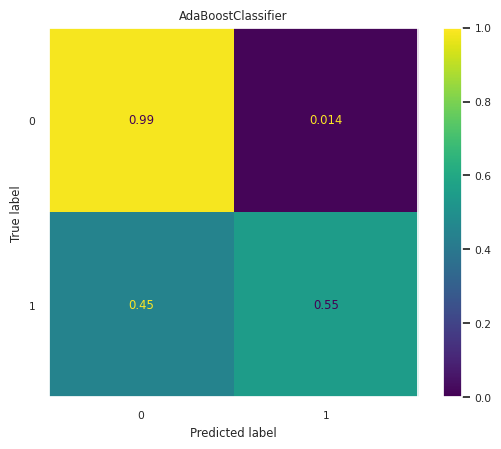
\includegraphics[width=\textwidth]{images/models/Ada_base.png}
        \caption{Baseline}
        %\label{fig:Ada_base}
    \end{subfigure}
    \begin{subfigure}[c]{0.4\textwidth}
        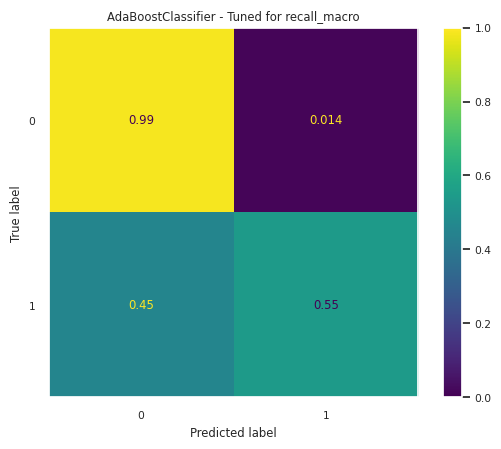
\includegraphics[width=\textwidth]{images/models/Ada_tuned.png}
        \caption{Tuned}
        %\label{fig:Ada_tuned}
    \end{subfigure}
    \caption{\subsecname\ results}
    %\label{fig:Ada_results}
\end{figure}
\end{frame}

\subsection{K-Nearest Neighbor}
\begin{frame}{\subsecname}
\begin{columns}
    \column{0.5\textwidth}
    \begin{table}
        \footnotesize
        \centering
        \begin{tabular}{ll}
            parameter & tuned value \\
            \hline\hline
            \txt{algorithm} & \txt{"kd_tree"} \\
            \txt{metric} & \txt{"manhattan"} \\
            \txt{leaf_size} & 40 \\
            \txt{n_neighbors} & 1 \\
        \end{tabular}
        %\label{tab:my_label}
    \end{table}
    \column{0.5\textwidth}
    \begin{table}
        \footnotesize
        \centering
        \begin{tabular}{lc}
            metric & result \\
            \hline\hline
            \txt{recall} (class 1) & 45\% \\
            \txt{recall_macro} & 72\% \\
        \end{tabular}
        %\label{tab:my_label}
    \end{table}
\end{columns}

\begin{figure}
    \centering
    \begin{subfigure}[c]{0.4\textwidth}
        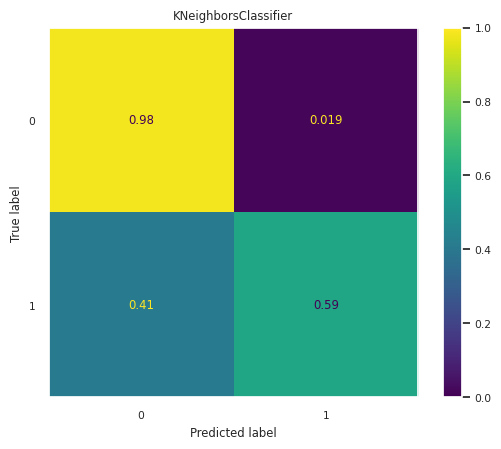
\includegraphics[width=\textwidth]{images/models/KNN_base.png}
        \caption{Baseline}
        %\label{fig:Ada_base}
    \end{subfigure}
    \begin{subfigure}[c]{0.4\textwidth}
        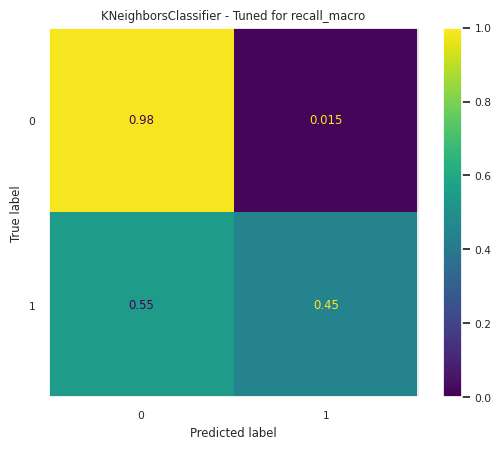
\includegraphics[width=\textwidth]{images/models/KNN_tuned.png}
        \caption{Tuned}
        %\label{fig:Ada_tuned}
    \end{subfigure}
    \caption{\subsecname\ results}
    %\label{fig:Ada_results}
\end{figure}
\end{frame}

\subsection{Gaussian Naive Bayes}
\begin{frame}{\subsecname}
\begin{columns}
    \column{0.5\textwidth}
    \begin{table}
        \footnotesize
        \centering
        \renewcommand{\arraystretch}{1.2}
        \begin{tabular}{ll}
            parameter & tuned value \\
            \hline\hline
            \txt{var_smoothing} & $10^{-8}$
        \end{tabular}
        %\label{tab:my_label}
    \end{table}
    \column{0.5\textwidth}
    \begin{table}
        \footnotesize
        \centering
        \begin{tabular}{lc}
            metric & result \\
            \hline\hline
            \txt{recall} (class 1) & 34\% \\
            \txt{recall_macro} & 66\% \\
        \end{tabular}
        %\label{tab:my_label}
    \end{table}
\end{columns}

\begin{figure}
    \centering
    \begin{subfigure}[c]{0.4\textwidth}
        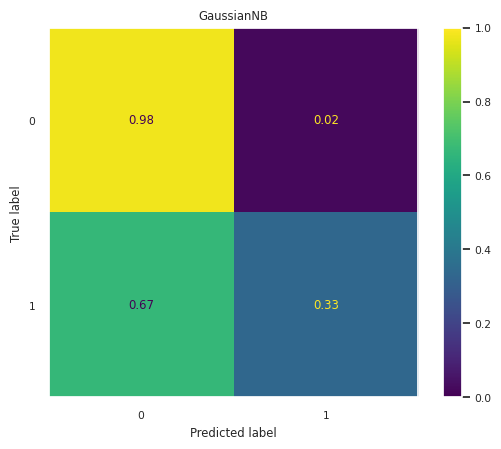
\includegraphics[width=\textwidth]{images/models/GNB_base.png}
        \caption{Baseline}
        %\label{fig:Ada_base}
    \end{subfigure}
    \begin{subfigure}[c]{0.4\textwidth}
        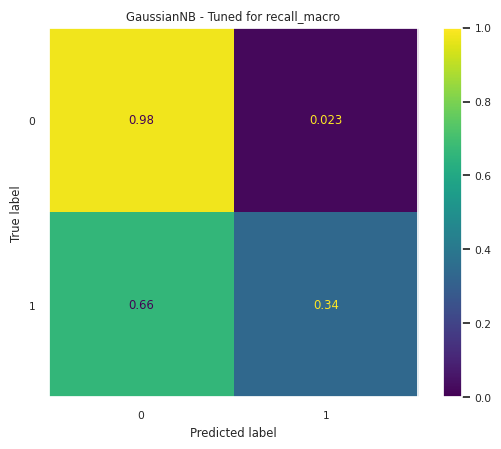
\includegraphics[width=\textwidth]{images/models/GNB_tuned.png}
        \caption{Tuned}
        %\label{fig:Ada_tuned}
    \end{subfigure}
    \caption{\subsecname\ results}
    %\label{fig:Ada_results}
\end{figure}
\end{frame}

\subsection{Perceptron}
\begin{frame}{\subsecname}
\begin{columns}
    \column{0.5\textwidth}
    \begin{table}
        \footnotesize
        \centering
        \begin{tabular}{ll}
            parameter & tuned value \\
            \hline\hline
            \txt{early_stopping} & \txt{True} \\
            \txt{penalty} & \txt{None} \\
            \txt{class_weight} & \txt{"balanced"} \\
            \txt{eta0} & 1.0 \\
        \end{tabular}
        %\label{tab:my_label}
    \end{table}
    \column{0.5\textwidth}
    \begin{table}
        \footnotesize
        \centering
        \begin{tabular}{lc}
            metric & result \\
            \hline\hline
            \txt{recall} (class 1) & 72\% \\
            \txt{recall_macro} & 79\% \\
        \end{tabular}
        %\label{tab:my_label}
    \end{table}
\end{columns}

\begin{figure}
    \centering
    \begin{subfigure}[c]{0.4\textwidth}
        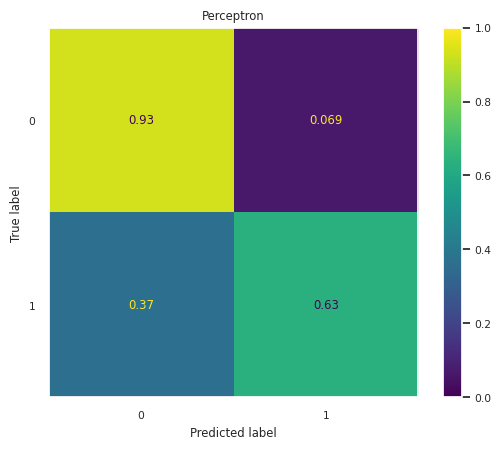
\includegraphics[width=\textwidth]{images/models/Percep_base.png}
        \caption{Baseline}
        %\label{fig:Ada_base}
    \end{subfigure}
    \begin{subfigure}[c]{0.4\textwidth}
        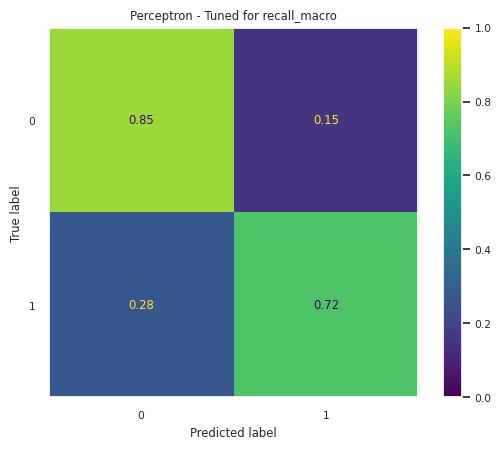
\includegraphics[width=\textwidth]{images/models/Percep_tuned.png}
        \caption{Tuned}
        %\label{fig:Ada_tuned}
    \end{subfigure}
    \caption{\subsecname\ results}
    %\label{fig:Ada_results}
\end{figure}
\end{frame}

\subsection{Support Vector Machine}
\begin{frame}{\subsecname}
\begin{columns}
    \column{0.5\textwidth}
    \begin{table}
        \scriptsize
        \centering
        \begin{tabular}{ll}
            parameter & tuned value \\
            \hline\hline
            \txt{kernel} & \txt{"poly"} \\
            \txt{class_weight} & \txt{"balanced"} \\
            \txt{shrinking} & \txt{False} \\
            \txt{gamma} & \txt{"auto"} \\
            \txt{C} & \txt{100} \\
        \end{tabular}
        %\label{tab:my_label}
    \end{table}
    \column{0.5\textwidth}
    \begin{table}
        \footnotesize
        \centering
        \begin{tabular}{lc}
            metric & result \\
            \hline\hline
            \txt{recall} (class 1) & 85\% \\
            \txt{recall_macro} & 88\% \\
        \end{tabular}
        %\label{tab:my_label}
    \end{table}
\end{columns}

\begin{figure}
    \centering
    \begin{subfigure}[c]{0.32\textwidth}
        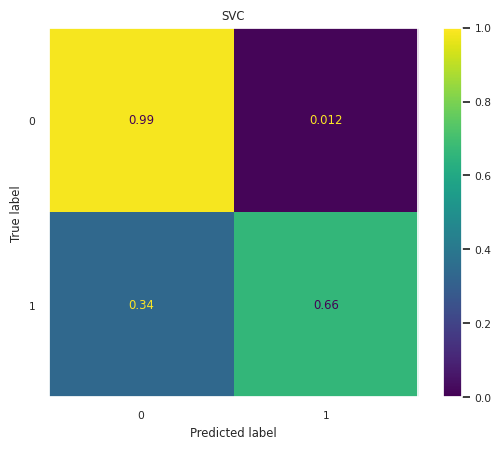
\includegraphics[width=\textwidth]{images/models/SVM_base.png}
        \caption{Baseline}
        %\label{fig:Ada_base}
    \end{subfigure}
    \begin{subfigure}[c]{0.32\textwidth}
        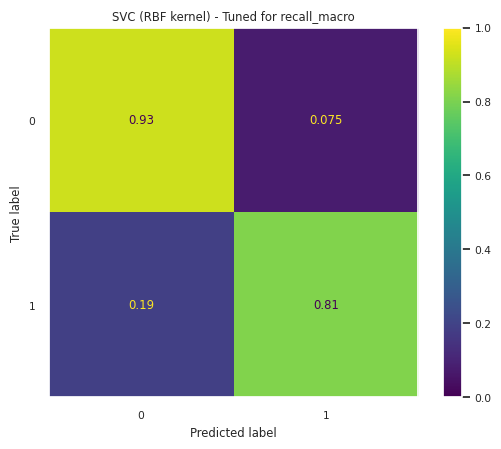
\includegraphics[width=\textwidth]{images/models/SVM_tuned_rbf.png}
        \caption{Tuned (RBF)}
        %\label{fig:Ada_tuned}
    \end{subfigure}
    \begin{subfigure}[c]{0.32\textwidth}
        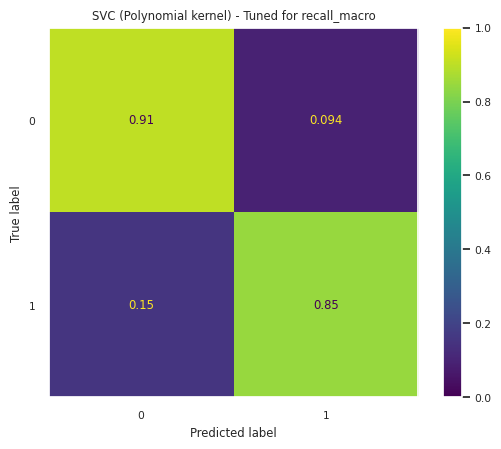
\includegraphics[width=\textwidth]{images/models/SVM_tuned_poly.png}
        \caption{Tuned (Polynomial)}
        %\label{fig:Ada_tuned}
    \end{subfigure}
    \caption{\subsecname\ results}
    %\label{fig:Ada_results}
\end{figure}
\end{frame}

\subsection{Gradient Descent}
\begin{frame}{\subsecname}
\begin{columns}
    \column{0.5\textwidth}
    \begin{table}
        \scriptsize
        \centering
        \begin{tabular}{ll}
            parameter & tuned value \\
            \hline\hline
            \txt{class_weight} & \txt{"balanced"} \\
            \txt{penalty} & \txt{"elasticnet"} \\
            \txt{learning_rate} & \txt{"invscaling"} \\
            \txt{loss} & \txt{"hinge"} \\
            \txt{alpha} & 1.0 \\
            \txt{eta0} & 0.1 \\
        \end{tabular}
        %\label{tab:my_label}
    \end{table}
    \column{0.5\textwidth}
    \begin{table}
        \footnotesize
        \centering
        \begin{tabular}{lc}
            metric & result \\
            \hline\hline
            \txt{recall} (class 1) & 80\% \\
            \txt{recall_macro} & 80\% \\
        \end{tabular}
        %\label{tab:my_label}
    \end{table}
\end{columns}
\vspace{-1.0em}
\begin{figure}
    \centering
    \begin{subfigure}[c]{0.4\textwidth}
        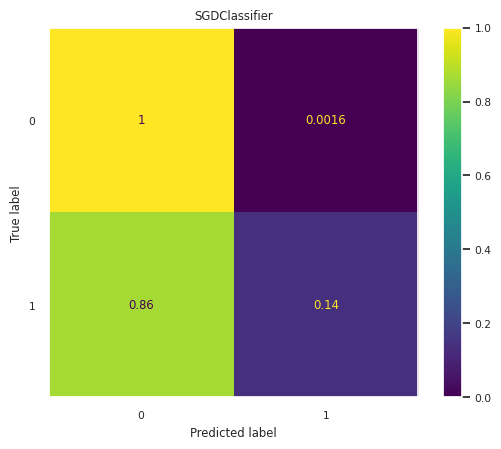
\includegraphics[width=\textwidth]{images/models/SGD_base.png}
        \caption{Baseline}
        %\label{fig:Ada_base}
    \end{subfigure}
    \begin{subfigure}[c]{0.4\textwidth}
        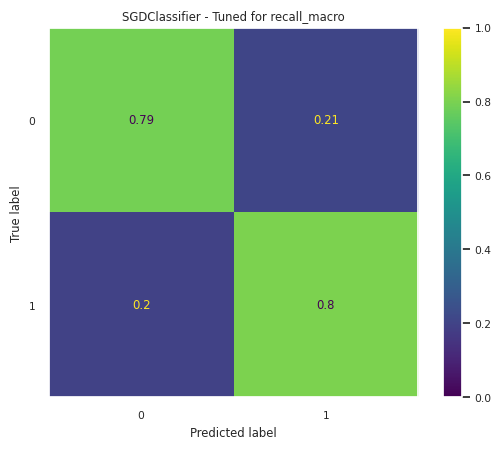
\includegraphics[width=\textwidth]{images/models/SGD_tuned.png}
        \caption{Tuned}
        %\label{fig:Ada_tuned}
    \end{subfigure}
    \caption{\subsecname\ results}
    %\label{fig:Ada_results}
\end{figure}
\end{frame}